%% Radiology: Artificial Intelligence submission draft
%% To compile: latexmk -pdf main_radiology_ai

\documentclass[11pt]{article}

\usepackage[margin=1in]{geometry}%
\usepackage{graphicx}%
\usepackage{multirow}%
\usepackage{amsmath,amssymb,amsfonts}%
\usepackage{xcolor}%
\usepackage{textcomp}%
\usepackage{booktabs}%
\usepackage{tabularx}%
\usepackage{flafter}%
\usepackage{placeins}%
\usepackage{float}%
\usepackage[numbers,sort&compress,round]{natbib}%
\renewcommand{\bibnumfmt}[1]{#1.}% AMA/NLM: reference list numbered "1." not "[1]"
\usepackage{url}%
\usepackage{hyperref}%
\usepackage{lineno}%
\usepackage{setspace}%
\setlength{\emergencystretch}{2em}
\Urlmuskip=0mu plus 1mu\relax
\hypersetup{hypertexnames=false}
\setcounter{topnumber}{3}
\setcounter{bottomnumber}{2}
\setcounter{totalnumber}{4}
\renewcommand{\topfraction}{0.88}
\renewcommand{\bottomfraction}{0.75}
\renewcommand{\textfraction}{0.08}
\setlength{\textfloatsep}{10pt plus 2pt minus 2pt}
\setlength{\floatsep}{8pt plus 2pt minus 2pt}

\newcolumntype{Y}{>{\raggedright\arraybackslash}X}
\newcommand{\keywords}[1]{\par\noindent\textbf{Keywords:} #1\par}
\providecommand{\bibcommenthead}{}

\raggedbottom

\begin{document}

\doublespacing
\pagestyle{empty}  % Radiology: AI — do not number manuscript pages

%% NOTE: Radiology: Artificial Intelligence uses double-blind peer review.
%% This is the BLINDED manuscript: no author names, affiliations, funding
%% details, or self-identifying links appear here. Author identifiers,
%% degrees, contributions, funding, and acknowledgements are on the
%% separate title page (title_page_radiology_ai.tex).

\begin{center}
{\LARGE\bfseries Metadata Reliance in Vision-Language Models\\
for CT Lung Nodule Malignancy Prediction\par}
\end{center}
\vspace{0.5em}

\begin{center}\textbf{Article Type: Original Research}\end{center}
\vspace{0.5em}

\noindent\textbf{Summary Statement:} \textbf{Structured prompt metadata, rather than computed tomography images alone, accounted for much of apparent vision-language-model performance in a retrospective lung nodule malignancy benchmark.}

\vspace{0.75em}
\noindent\textbf{Key Points}
\begin{itemize}
\item In 917 LUNA25 nodules, visual-only Gemini~3 Flash prompting achieved AUC 0.682--0.712; adding structured metadata raised the strongest condition to AUC 0.739, while a matched text-only control reached AUC 0.693.
\item In a sparse-montage audit, Claude Opus~4.8 and Gemini~3.1 Pro rose from near-chance image-only performance to metadata-assisted AUCs of 0.730 and 0.729, respectively; GPT-5.5 image-only outputs were retained only as an interface-provenance check.
\item The strongest metadata-assisted vision-language model remained below CT-only supervised three-dimensional deep learning, with AUC 0.739 versus 0.872 for STU-Net.
\end{itemize}

\newpage
\begin{abstract}
\textbf{Purpose:} To determine whether general-purpose vision-language model (VLM) performance for CT lung nodule malignancy prediction reflects visual interpretation or prompt-supplied structured metadata.
\textbf{Materials and Methods:} This retrospective benchmark used LUNA25 (917 annotations from 318 patients; 81 malignant) and LNDb external validation (814 rows; 74 malignant). Gemini~3 Flash Preview underwent six prompt/input conditions plus a matched text-only control. Hosted VLM inference was performed on April~30, 2026. Claude Opus~4.8 and Gemini~3.1 Pro were evaluated in a zero-shot sparse-montage audit; GPT-5.5 metadata-assisted and text-only rows were reported separately because image-only delivery failed in the tested interface. Comparators were seven supervised 3-D deep-learning (DL) models, Brock, and structured-metadata baselines; performance was assessed with ROC-AUC and paired DeLong testing.
\textbf{Results:} Visual-only Gemini conditions reached AUC 0.682--0.712; adding structured metadata raised the 20-shot rich condition to AUC 0.739. The matched text-only control reached AUC 0.693, and F3 exceeded F0 by 0.047 AUC units (paired DeLong $P=.02$). In the sparse-montage audit, metadata increased AUC by 0.233 for Claude Opus~4.8 and 0.213 for Gemini~3.1 Pro; text-only controls recovered most metadata-assisted signal. The strongest VLM setting remained below supervised 3-D DL (best AUC, 0.872; $P<.001$). On LNDb, visual-only Gemini remained below all seven DL baselines.
\textbf{Conclusion:} Prompt-supplied structured metadata accounted for substantial apparent VLM performance in this retrospective CT lung nodule benchmark. Text-only and metadata-control conditions are needed when evaluating multimodal VLMs with structured clinical descriptors.
\end{abstract}

\keywords{vision-language model, lung nodule, malignancy prediction, chest CT, metadata reliance, external validation}

\section*{Abbreviations}
\noindent AUC = area under the receiver operating characteristic curve; CT = computed tomography; DL = deep learning; ECE = expected calibration error; HU = Hounsfield unit; PR-AUC = precision--recall area under the curve; VLM = vision-language model.

%%==================================================================%%
%% Introduction                                                      %%
%%==================================================================%%
\linenumbers
\section{Introduction}\label{sec:intro}

Lung cancer screening with low-dose CT reduces mortality in high-risk populations, but characterization of screen-detected pulmonary nodules remains difficult because benign and malignant nodules overlap in appearance~\citep{ref-nlst,ref-fleischner}. Supervised 3-D deep-learning (DL) models trained directly on volumetric CT labels can perform well on this task~\citep{ref-venkadesh}, while general-purpose vision-language models (VLMs) and radiology foundation models are increasingly proposed as flexible clinical imaging assistants~\citep{ref-lee2025review3d,ref-wu2025radfm,ref-wu2025vlfm3d}.

For volumetric CT, however, apparent VLM accuracy may combine image interpretation with signals supplied in the prompt. Recent medical VLM evaluations have emphasized that high aggregate accuracy can conceal shortcut behavior, robustness failures, and benchmark-interface artifacts~\citep{ref-jin2024hidden,ref-kurz2025benchmark,ref-cheng2025robustness}. Lung nodule prompts often include structured descriptors such as size, margin, attenuation, smoking status, and location; these variables are themselves diagnostic predictors and overlap with established clinical rules such as Brock. Without text-only and metadata-aware controls, metadata-assisted VLM performance can be mistaken for visual CT reasoning.

We audited this issue for CT lung nodule malignancy prediction using LUNA25 and LNDb. We combined a deep Gemini~3 Flash Preview prompt/input ablation, a matched text-only control, a cross-family sparse-montage audit in Claude Opus~4.8, Gemini~3.1 Pro, and GPT-5.5, and comparisons with supervised 3-D DL, Brock, and structured-metadata baselines. We hypothesized that VLMs would show nontrivial signal but remain below task-specific 3-D DL, and that a substantial fraction of metadata-assisted VLM performance would be recoverable without images.

%%==================================================================%%
%% Materials and Methods                                             %%
%%==================================================================%%
\section{Materials and Methods}\label{sec:methods}

\subsection{Study Design and Data}

Because this retrospective computational benchmark used public, de-identified datasets, institutional review board approval and informed consent were not required (Figure~\ref{fig:overview}). Reporting was aligned with CLAIM, STARD-AI, and TRIPOD-AI/LLM principles for AI diagnostic and prediction-model studies~\citep{ref-claim,ref-stard-ai,ref-tripod-ai,ref-tripod-llm}. The internal test set was the fixed patient-disjoint LUNA25 test split (917 annotations from 318 patients; 81 malignant, 836 benign) derived from NLST nodule-centered CT crops~\citep{peeters2025luna25ann,peeters2025luna25img}. Structured prompt fields included LUNA25 nodule descriptors and matched NLST demographic/smoking fields. Self-reported race was included in the primary Z3/F3 clinical text because it was present in the matched NLST descriptors; race-excluded tabular sensitivity analyses are reported separately. External validation used the DL-matched LNDb 814-row sheet (740 benign, 74 malignant; 439 unique findings)~\citep{pedrosa2019lndb}.

\subsection{VLM Inputs and Controls}

For the primary Gemini experiments, each $64\times128\times128$ CT crop was clipped to $[-1000,1000]$ HU and encoded as a 20-fps MP4 video following the CT-to-video approach of Xu et al.~\citep{ref-xu2026}. Gemini~3 Flash Preview was tested under six conditions: Z1/Z2/Z3 for zero-shot minimal, rich, and rich+clinical prompts, and F1/F2/F3 for the corresponding 20-shot conditions. F0 was a matched text-only control retaining the F3 prompt scaffold, exemplar labels/text, target clinical text, JSON schema, model identifier, and temperature, but removing all CT videos. Z0 was reserved for the zero-shot metadata-only condition in the cross-family sparse-montage audit, where no exemplar text or CT image was provided. Hosted VLM inference was performed on April~30, 2026. Calls used temperature~0 where supported and required a JSON response with a malignancy confidence score and one-sentence rationale; compact condition definitions and input routes are provided in the Supplement, and exact model identifiers, serialized prompt templates, software versions, and parsed outputs are provided in the anonymized review repository. Four additional F3 repeats formed the averaged F3A sensitivity estimate. Gemini~2.5 Flash, Gemini~2.5 Pro, Gemini~3.1 Pro Preview, and MedGemma~1.5-4B were evaluated under F3 for context.

For the cross-family audit, Claude Opus~4.8, Gemini~3.1 Pro Preview, and GPT-5.5 were evaluated through the same hosted model interface using Z2 image-only, Z3 image+metadata, and Z0 metadata-only prompts. Image rows used a standardized axial montage of frames 9, 29, and 49 from each 64-frame clip, matching the sparse frame positions observed in the hosted Gemini video sampling probe. The same montage audit was also run for Gemini~3 Flash Preview as a bridge to the primary video-input ablation. Matching frame indices does not make the montage pixel-token equivalent to native video ingestion, because the three frames are concatenated into a single image and may undergo different resizing, layout parsing, and modality-specific preprocessing. This audit was designed to test whether metadata reliance generalized across hosted VLM interfaces under a portable sparse visual input, not to rank vendor-native image or video ingestion. GPT-5.5 image-only responses were constant at 0.5 with no-image rationales and were retained only as an interface-provenance check.

\subsection{Comparators and Statistical Analysis}

Seven supervised DL baselines were trained/evaluated on the same LUNA25 split: ResNet-18/50~\citep{ref-resnet}, DenseNet-121~\citep{ref-densenet}, EfficientNet-B0~\citep{ref-efficientnet}, STU-Net~\citep{ref-stunet}, ViT-Base~\citep{ref-vit}, and Swin-UNETR~\citep{ref-swin-unetr}. We also evaluated exploratory 20-shot Med3D ResNet18+TTT variants~\citep{ref-sun2024ttt}, the parsimonious Brock model~\citep{ref-mcwilliams} on 701 cases with complete mappable metadata, and classical structured-metadata models trained on the LUNA25 training split. The primary endpoint was ROC-AUC. The primary contrasts were F3 versus F0 and F3 versus the strongest supervised CT-only baseline. Pairwise AUC comparisons used paired DeLong tests~\citep{ref-delong}; 95\% CIs used stratified bootstrap resampling, with patient-cluster and LNDb finding-cluster sensitivity analyses. Other DeLong tests, calibration, PR-AUC, decision-curve net benefit~\citep{ref-vickers}, subgroup analyses, and rationale audits were exploratory and were not adjusted for multiplicity. Analyses were performed in Python~3 using scikit-learn, SciPy, NumPy, and pandas, with matplotlib for figures; a paired DeLong implementation was used for AUC comparisons, and two-sided $P<.05$ denoted statistical significance. Pinned package versions, per-sample outputs, and scripts are released.

%%==================================================================%%
%% Results                                                           %%
%%==================================================================%%
\section{Results}\label{sec:results}

\begin{figure}[!t]
\centering
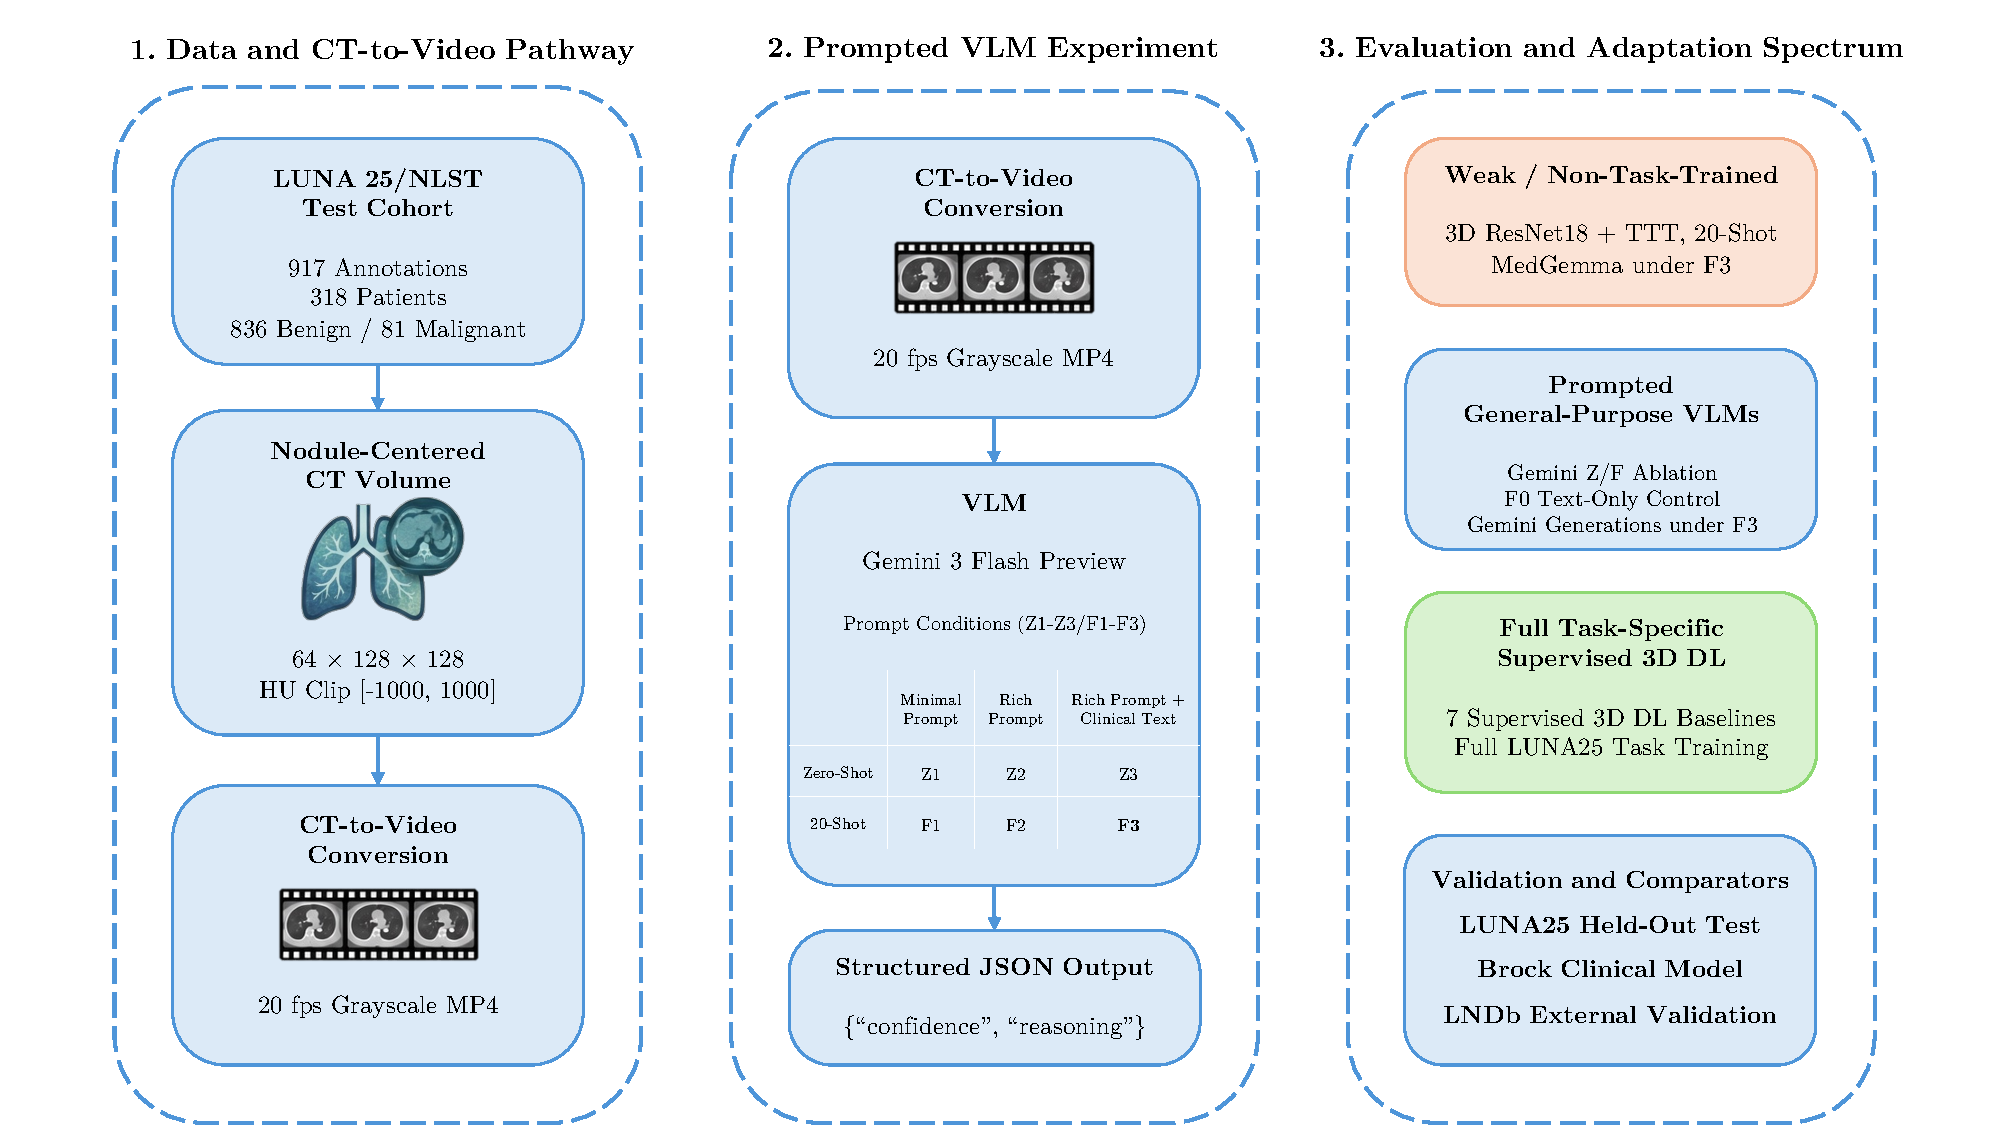
\includegraphics[width=\linewidth]{../figures/fig1_overview.pdf}
\caption{Study design and evaluation pipeline. Prompt/input conditions are labelled Z1--Z3 for zero-shot prompts (minimal, rich, rich+clinical), F1--F3 for the corresponding 20-shot conditions, and F0 for the matched F3 text-only control. Z0 denotes the separate zero-shot metadata-only control used in the cross-family sparse-montage audit.}\label{fig:overview}
\end{figure}

\subsection{Gemini Prompt/Input Ablation}

The LUNA25 test set included 917 nodules; mean age was 62.6 years, 182/318 patients (57.2\%) were male, and 150/318 were current smokers. Visual-only Gemini conditions clustered at AUC 0.682--0.712 (Table~\ref{tab:ablation}; Figure~\ref{fig:roc}). Adding structured clinical text raised the strongest setting, Gemini F3, to AUC 0.739 (95\% CI: 0.677, 0.798), while the matched F0 text-only control reached AUC 0.693 (95\% CI: 0.634, 0.746). F3 exceeded F0 by 0.047 AUC units (paired DeLong $P=.02$), but F0 correlated more strongly with Brock probability ($\rho=0.723$) than image-only F2 ($\rho=0.147$), indicating substantial structured-text signal. Cross-generation F3 runs were similar for Gemini~3 Flash Preview and Gemini~3.1 Pro Preview (AUC 0.739 vs 0.736), lower for Gemini~2.5 models (AUC 0.682--0.710), and lower for MedGemma~1.5-4B (AUC 0.594).

\begin{table}[!htbp]
\caption{Gemini~3 Flash Preview prompt/input ablation on LUNA25.}\label{tab:ablation}
\small
\setlength{\tabcolsep}{4pt}
\begin{tabularx}{\textwidth}{@{}Yccccc@{}}
\toprule
Condition & CT video & Clinical text & Shots & AUC & 95\% CI \\
\midrule
Z1 minimal & Yes & No & 0 & 0.702 & 0.639--0.762 \\
Z2 rich & Yes & No & 0 & 0.682 & 0.615--0.746 \\
Z3 rich+clinical & Yes & Yes & 0 & 0.730 & 0.671--0.783 \\
F1 minimal & Yes & No & 20 & 0.712 & 0.661--0.767 \\
F2 rich & Yes & No & 20 & 0.699 & 0.638--0.756 \\
\textbf{F3 rich+clinical} & Yes & Yes & 20 & \textbf{0.739} & 0.677--0.798 \\
F0 text-only & No & Yes & 20 & 0.693 & 0.634--0.746 \\
\bottomrule
\end{tabularx}
\par\vspace{3pt}\footnotesize Z denotes zero-shot and F denotes 20-shot/few-shot. F0 retained the F3 text scaffold and exemplar labels/text but removed all CT videos. F3 versus F0 paired DeLong $P=.02$.
\end{table}

\begin{figure}[tb]
\centering
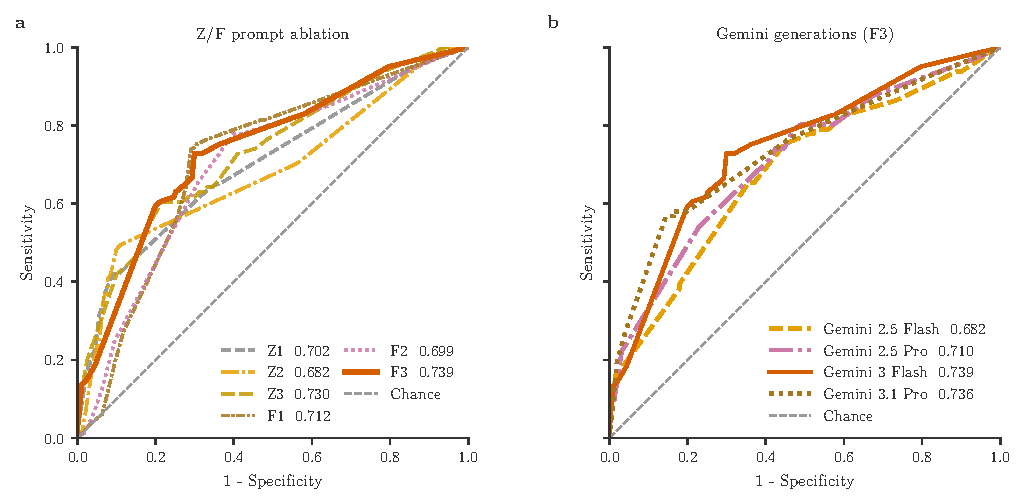
\includegraphics[width=\linewidth]{../figures/fig2_roc.pdf}
\caption{Receiver operating characteristic curves for the Gemini~3 Flash Preview Z/F prompt ablation and the Gemini-generation F3 comparison.}\label{fig:roc}
\end{figure}

\subsection{Cross-Family Metadata Audit}

Under the standardized three-slice montage, image-only performance was near chance for the Gemini~3 Flash bridge (AUC 0.508), Claude Opus~4.8 (AUC 0.497), and Gemini~3.1 Pro (AUC 0.516), whereas adding structured metadata raised these rows to AUC 0.72--0.73 (Table~\ref{tab:crossfamily}). Text-only controls recovered most of the metadata-assisted signal (AUC 0.721, 0.719, and 0.713, respectively). Brock correlations rose from near zero in image-only rows to 0.77--0.84 after metadata was added. GPT-5.5 image-plus-text and text-only rows were similar (AUC 0.712 and 0.703), but its image-only row was not interpreted because the interface did not appear to deliver the image.

\begin{table}[!htbp]
\caption{Cross-family zero-shot sparse-montage audit on LUNA25.}\label{tab:crossfamily}
\scriptsize
\setlength{\tabcolsep}{3pt}
\begin{tabularx}{\textwidth}{@{}Ycccccc@{}}
\toprule
Model & $n_{\mathrm{pair}}$ & Z2 & Z3 & Lift & Z0 & $\rho_{\mathrm{Brock}}$ Z2/Z3 \\
\midrule
Gemini~3 Flash video reference & 917 & 0.682 & 0.730 & $+0.047$ & -- & 0.18/0.64 \\
Gemini~3 Flash montage & 917 & 0.508 & 0.722 & $+0.214$ & 0.721 & $-0.01$/0.77 \\
Claude Opus~4.8 & 917 & 0.497 & 0.730 & $+0.233$ & 0.719 & $-0.01$/0.84 \\
Gemini~3.1 Pro & 917 & 0.516 & 0.729 & $+0.213$ & 0.713 & 0.06/0.79 \\
GPT-5.5 & 917 & 0.500\textsuperscript{\ddag} & 0.712 & NA\textsuperscript{\ddag} & 0.703 & NA/0.82 \\
\bottomrule
\end{tabularx}
\par\vspace{3pt}\footnotesize Z2=rich image-only, Z3=rich image+metadata, Z0=metadata-only. The video-reference row uses the original Gemini video-input ablation; other rows use the standardized single-image three-slice montage. The video-reference and montage rows share the nominal sampled frame positions but differ in ingestion path and preprocessing. Paired Z2-versus-Z3 DeLong $P$ values for interpretable image-delivery rows were $.23$, ${<}.001$, ${<}.001$, and ${<}.001$, respectively. \textsuperscript{\ddag}GPT-5.5 image-only responses were constant 0.5 with no-image rationales, indicating failed image delivery in the tested interface; this row was not included in image-only, lift, or paired Z2-versus-Z3 interpretation.
\end{table}

\subsection{Comparison with Supervised DL, Brock, and External Validation}

Full-data supervised 3-D DL remained strongest (Table~\ref{tab:vsdl}; Figure~\ref{fig:bar}). Gemini F3 received both CT video and structured metadata, while DL baselines used CT only; nevertheless, Gemini F3 was below six of seven DL baselines. The paired AUC gap was $-0.133$ versus STU-Net (AUC 0.872; DeLong $P<.001$) and $-0.124$ versus EfficientNet-B0 (AUC 0.863; DeLong $P<.001$). On the 701 Brock-computable cases, Brock reached AUC 0.774 and Gemini F3 reached AUC 0.750 (DeLong $P=.40$). A structured-only gradient-boosting model reached AUC 0.710, overlapping the visual-only Gemini plateau and exceeding F0 text-only prompting.

\begin{table}[tb]
\caption{Performance spectrum on LUNA25.}\label{tab:vsdl}
\small
\setlength{\tabcolsep}{4pt}
\begin{tabularx}{\textwidth}{@{}Y>{\raggedright\arraybackslash}p{0.14\textwidth}cc@{}}
\toprule
Method & Type & AUC & 95\% CI \\
\midrule
STU-Net & DL & 0.872 & 0.833--0.906 \\
EfficientNet-B0 & DL & 0.863 & 0.827--0.898 \\
ResNet-18 & DL & 0.856 & 0.823--0.887 \\
DenseNet-121 & DL & 0.833 & 0.789--0.874 \\
ResNet-50 & DL & 0.817 & 0.782--0.848 \\
Swin-UNETR & DL & 0.800 & 0.752--0.846 \\
\textbf{Gemini F3} & \textbf{GP-VLM} & \textbf{0.739} & 0.677--0.798 \\
ViT-Base & DL & 0.693 & 0.635--0.744 \\
MedGemma 1.5-4B (F3) & Spec.\ VLM & 0.594 & 0.555--0.630 \\
20-shot Med3D ResNet18+TTT & Weak DL & 0.558--0.592 & observed range \\
\bottomrule
\end{tabularx}
\par\vspace{3pt}\footnotesize GP-VLM=general-purpose VLM; Spec.\ VLM=specialty medical-imaging VLM. DL baselines used CT volumes only; Gemini F3 additionally received structured metadata.
\end{table}

\begin{figure}[tb]
\centering
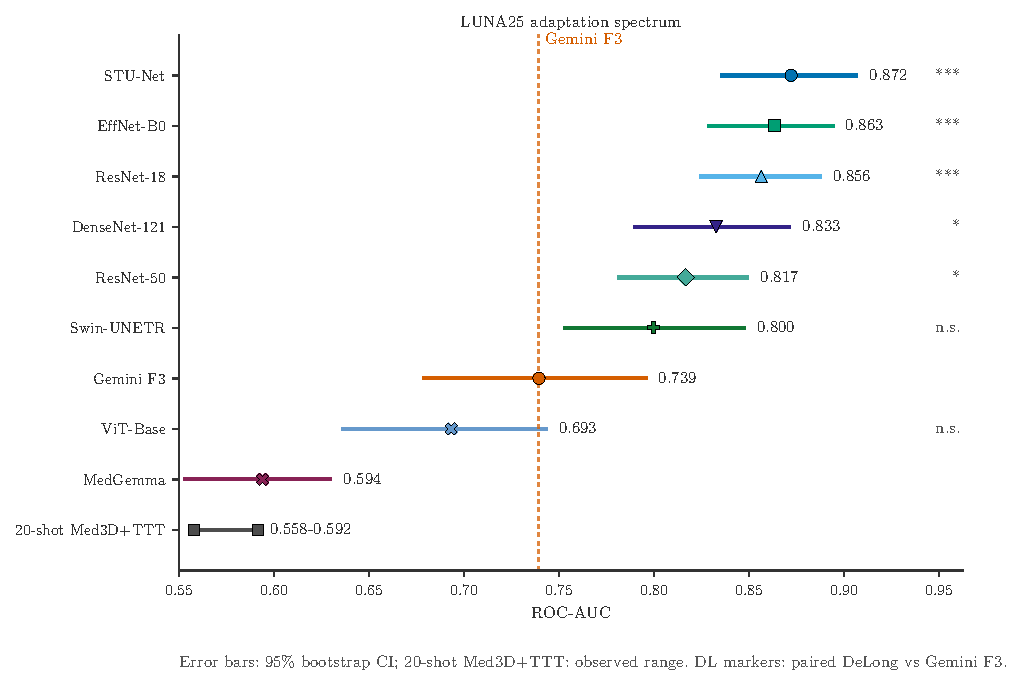
\includegraphics[width=\linewidth]{../figures/fig3_bar.pdf}
\caption{Performance spectrum on LUNA25. Points and error bars show AUCs with 95\% bootstrap CIs for supervised DL baselines, Gemini F3, MedGemma~1.5-4B, and weak-adaptation Med3D ResNet18+TTT variants. Stars denote paired DeLong tests versus Gemini F3: *$P<.05$, **$P<.01$, ***$P<.001$; n.s.=not significant.}\label{fig:bar}
\end{figure}

Decision-curve and calibration analyses supported the discrimination results. STU-Net had higher PR-AUC than Gemini F3 (0.520 vs 0.252), and raw-score net benefit at a 10\% threshold was $+0.031$ for STU-Net and $+0.003$ for Gemini F3 (Supplement). Gemini F3 was poorly calibrated (Brier 0.222, ECE 0.270), whereas STU-Net combined higher AUC with lower Brier score (0.090). At threshold 0.5, Gemini F3 misclassified 280/917 cases; representative discordant cases are shown in Figure~\ref{fig:failure}.

\begin{figure}[tb]
\centering
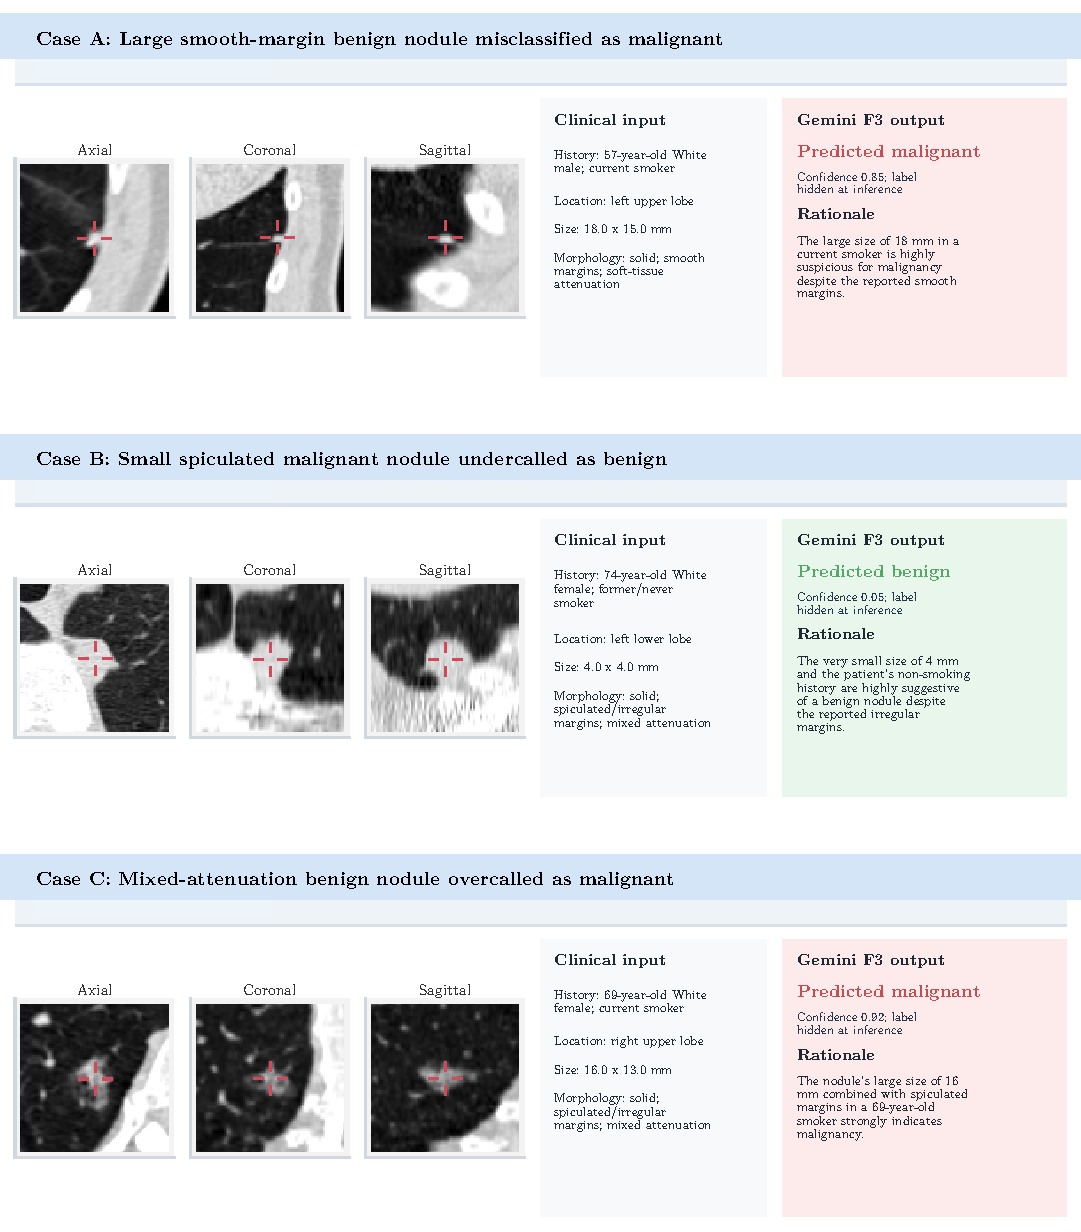
\includegraphics[width=0.88\linewidth]{../figures/fig4_failure.pdf}
\caption{Representative discordant Gemini F3 cases on LUNA25. Each panel shows orthogonal CT views, supplied clinical input, emitted confidence and rationale, and the reference label for the F3 condition.}\label{fig:failure}
\end{figure}

On LNDb, where comparable structured metadata were unavailable, visual-only Gemini prompting remained below all seven DL baselines (Table~\ref{tab:lndb}). Gemini F2 reached AUC 0.654 and Gemini Z2 reached AUC 0.642; EfficientNet-B0 reached AUC 0.815 and exceeded Gemini F2 by 0.161 AUC units (paired DeLong $P<.001$). The qualitative ranking was unchanged under finding-cluster bootstrap.

\begin{table}[!ht]
\caption{External validation on LNDb using the DL-matched 814-row evaluation sheet.}\label{tab:lndb}
\small
\setlength{\tabcolsep}{4pt}
\begin{tabularx}{\textwidth}{@{}Ycccc@{}}
\toprule
Method & Int. AUC & LNDb AUC & Row 95\% CI & Cluster 95\% CI \\
\midrule
EfficientNet-B0 & 0.863 & 0.815 & 0.761--0.863 & 0.760--0.866 \\
ResNet-18 & 0.856 & 0.812 & 0.759--0.864 & 0.750--0.865 \\
DenseNet-121 & 0.833 & 0.807 & 0.754--0.858 & 0.746--0.861 \\
STU-Net & 0.872 & 0.803 & 0.742--0.863 & 0.740--0.862 \\
ResNet-50 & 0.817 & 0.762 & 0.706--0.816 & 0.701--0.821 \\
ViT-Base & 0.693 & 0.683 & 0.624--0.743 & 0.612--0.750 \\
Swin-UNETR & 0.800 & 0.666 & 0.596--0.728 & 0.592--0.737 \\
Gemini F2 & 0.699 & 0.654 & 0.592--0.715 & 0.587--0.724 \\
Gemini Z2 & 0.682 & 0.642 & 0.575--0.704 & 0.569--0.706 \\
\bottomrule
\end{tabularx}
\par\vspace{3pt}\footnotesize LNDb contained 740 benign and 74 malignant rows representing 439 unique findings. VLM external runs used visual-only Z2/F2 prompts because comparable structured clinical fields were unavailable.
\end{table}

%%==================================================================%%
%% Discussion                                                        %%
%%==================================================================%%
\section{Discussion}\label{sec:discussion}

This benchmark shows that general-purpose VLMs can produce moderate malignancy scores for CT lung nodules, but that their strongest apparent performance was materially influenced by prompt-supplied structured metadata. Visual-only Gemini conditions plateaued near AUC 0.70, whereas adding structured descriptors raised AUC to 0.739. A matched text-only control recovered much of the signal and was strongly aligned with Brock probability, indicating that the model could exploit tabular/radiologic descriptors without CT images.

The cross-family audit supports the same interpretation beyond Gemini video prompting. With identical three-slice montage input, the Gemini~3 Flash bridge, Claude Opus~4.8, and Gemini~3.1 Pro were near chance without metadata but rose to AUC 0.72--0.73 when metadata were added; their text-only controls recovered most of this gain. GPT-5.5 metadata-assisted and text-only rows showed the same approximate range, but its image-only row was retained only as an interface-provenance check because image delivery failed in the tested interface. For Gemini~3 Flash, the gap between native-video Z2 and montage Z2 despite matched nominal frame positions suggests that frame selection alone does not define the visual input: native video ingestion and single-image montage presentation can allocate visual detail differently. The key result is the convergence of metadata-assisted video, metadata-assisted montage, and text-only scores near AUC 0.72--0.73. This was not intended as a vendor leaderboard, because image/video ingestion differs across model families. Its value is narrower but clinically important: metadata reliance can masquerade as multimodal diagnostic performance across more than one frontier VLM family.

Task-specific supervised 3-D DL remained stronger. The comparison favored the VLM because Gemini F3 received CT video, 20 examples, and structured descriptors, whereas DL baselines used CT volume only. Even so, Gemini F3 was below six of seven DL baselines, had lower PR-AUC and net benefit than STU-Net, and was poorly calibrated. On LNDb, where comparable structured metadata were unavailable, visual-only Gemini remained below all DL baselines, reinforcing that metadata-assisted internal performance should not be generalized as visual CT competence.

Several limitations should be considered. LUNA25 labels combine pathology and longitudinal follow-up, and the deep ablation used one primary VLM family on one internal public cohort. The cross-family audit used a standardized three-frame montage rather than full 3-D CT or vendor-native video; even when sampled frame positions were matched to the Gemini video probe, montage and video inputs may differ in resizing, token allocation, and modality-specific preprocessing. GPT-5.5 image-only behavior suggested failed image delivery through that interface. Non-F3 VLM conditions were single runs, and calibration, subgroup, decision-curve, rationale, and weak-adaptation analyses were exploratory. We did not run metadata-permuted VLM inputs because deliberately mismatching descriptors and CTs is not a clinically meaningful diagnostic request. Self-reported race was included as an available NLST descriptor in Z3/F3 text; race-excluded tabular sensitivity analyses changed AUC minimally, but no powered VLM fairness audit was performed.

In conclusion, VLM evaluation for medical imaging should include metadata controls when prompts contain structured clinical or radiologic descriptors. For CT lung nodule malignancy prediction, the tested VLMs did not match supervised 3-D DL and should not be used as standalone diagnostic models. A more plausible near-term role is as an interface or reporting layer around validated imaging models, tested prospectively with calibration and clinical workflow endpoints.

%%==================================================================%%
%% Back matter                                                       %%
%%==================================================================%%
\section*{Data and code availability}
LUNA25 is publicly available at \url{https://luna25.grand-challenge.org/}. The LNDb ROI external-validation labels and the 814-row 10:1 evaluation sheet used here are derived from the public LNDb cohort; raw CT data are not redistributed and should be obtained from LUNA25 and LNDb under their respective terms. Per-sample VLM and DL predictions (JSONL/CSV), cross-family audit outputs, the row-level LNDb external-validation CSV, the Brock prediction file, prompts, exemplar identifiers, and all code (CT-to-video conversion, prompt construction, inference orchestration, cross-family shard merging and analysis, the Brock implementation, and the statistical, calibration, decision-curve, and figure-generation scripts, with pinned package versions) are available in an anonymized review repository and will be made public under the Apache~2.0 license on acceptance. \emph{[Repository link withheld for double-blind review; provided to editors and added on acceptance.]}

\section*{Funding and acknowledgements}
\emph{[Withheld for double-blind review; provided on the separate title page.]}

\section*{Competing interests}
The authors declare no competing interests.

\section*{Generative AI statement}
During preparation of this work, the authors used Anthropic Claude and OpenAI GPT-family models for language polishing, consistency checks, and non-substantive organizational suggestions after all analyses were completed. After using these tools, the authors reviewed and edited the content as needed and take full responsibility for the content of the publication. No AI tool generated new data, executed analyses, or created numerical results.

%%==================================================================%%
%% Bibliography (AMA/NLM style, hand-formatted in citation order)    %%
%% Not BibTeX-generated; refs.bib retained for the archived versions.%%
%%==================================================================%%
\begin{thebibliography}{99}

\bibitem{ref-nlst}
National Lung Screening Trial Research Team. Reduced lung-cancer mortality with low-dose computed tomographic screening. N Engl J Med. 2011;365(5):395-409. doi:10.1056/NEJMoa1102873

\bibitem{ref-fleischner}
MacMahon H, Naidich DP, Goo JM, et al. Guidelines for management of incidental pulmonary nodules detected on CT images: from the Fleischner Society 2017. Radiology. 2017;284(1):228-243. doi:10.1148/radiol.2017161659

\bibitem{ref-venkadesh}
Venkadesh KV, Setio AAA, Schreuder A, et al. Deep learning for malignancy risk estimation of pulmonary nodules detected at low-dose screening CT. Radiology. 2021;300(2):438-447. doi:10.1148/radiol.2021204433

\bibitem{ref-lee2025review3d}
Lee JO, Zhou HY, Berzin TM, Sodickson DK, Rajpurkar P. Multimodal generative AI for interpreting 3D medical images and videos. NPJ Digit Med. 2025;8:273. doi:10.1038/s41746-025-01649-4

\bibitem{ref-wu2025radfm}
Wu C, Zhang X, Zhang Y, Hui H, Wang Y, Xie W. Towards generalist foundation model for radiology by leveraging web-scale 2D\&3D medical data. Nat Commun. 2025;16:7866. doi:10.1038/s41467-025-62385-7

\bibitem{ref-wu2025vlfm3d}
Wu J, Wang Y, Zhong Z, et al. Vision-language foundation model for 3D medical imaging. NPJ Artif Intell. 2025;1:17. doi:10.1038/s44387-025-00015-9

\bibitem{ref-jin2024hidden}
Jin Q, Chen F, Zhou Y, et al. Hidden flaws behind expert-level accuracy of multimodal GPT-4 vision in medicine. NPJ Digit Med. 2024;7:190. doi:10.1038/s41746-024-01185-7

\bibitem{ref-kurz2025benchmark}
Kurz CF, Merzhevich T, Eskofier BM, Kather JN, Gmeiner B. Benchmarking vision-language models for diagnostics in emergency and critical care settings. NPJ Digit Med. 2025;8:423. doi:10.1038/s41746-025-01837-2

\bibitem{ref-cheng2025robustness}
Cheng Z, Ong AY, Wagner SK, et al. Understanding the robustness of vision-language models to medical image artefacts. NPJ Digit Med. 2025;8:727. doi:10.1038/s41746-025-02108-w

\bibitem{ref-claim}
Tejani AS, Klontzas ME, Gatti AA, et al. Checklist for Artificial Intelligence in Medical Imaging (CLAIM): 2024 update. Radiol Artif Intell. 2024;6(4):e240300. doi:10.1148/ryai.240300

\bibitem{ref-stard-ai}
Sounderajah V, Guni A, Liu X, et al. The STARD-AI reporting guideline for diagnostic accuracy studies using artificial intelligence. Nat Med. 2025;31:3283-3289. doi:10.1038/s41591-025-03953-8

\bibitem{ref-tripod-ai}
Collins GS, Moons KGM, Dhiman P, et al. TRIPOD+AI statement: updated guidance for reporting clinical prediction models that use regression or machine learning methods. BMJ. 2024;385:e078378. doi:10.1136/bmj-2023-078378

\bibitem{ref-tripod-llm}
Gallifant J, Afshar M, Ameen S, et al. The TRIPOD-LLM reporting guideline for studies using large language models. Nat Med. 2025;31:60-69. doi:10.1038/s41591-024-03425-5

\bibitem{peeters2025luna25ann}
Peeters D, Obreja B, Antonissen N, Jacobs C. The LUNA25 challenge: public training and development set---annotation data (1.0.0) [data set]. Zenodo; 2025. doi:10.5281/zenodo.14673658

\bibitem{peeters2025luna25img}
Peeters D, Obreja B, Antonissen N, Jacobs C. The LUNA25 challenge: public training and development set---imaging data (1.0.0) [data set]. Zenodo; 2025. doi:10.5281/zenodo.14223624

\bibitem{pedrosa2019lndb}
Pedrosa J, Aresta G, Ferreira C, et al. LNDb: a lung nodule database on computed tomography. arXiv:1911.08434 [preprint]. 2019.

\bibitem{ref-xu2026}
Xu N, He Q, Wang L, et al. Predicting invasiveness of lung adenocarcinoma from chest CT with few-shot vision-language ternary classification model. NPJ Digit Med. 2026;9:60. doi:10.1038/s41746-025-02229-2

\bibitem{ref-resnet}
He K, Zhang X, Ren S, Sun J. Deep residual learning for image recognition. In: Proceedings of the IEEE Conference on Computer Vision and Pattern Recognition (CVPR). 2016:770-778.

\bibitem{ref-densenet}
Huang G, Liu Z, Van Der Maaten L, Weinberger KQ. Densely connected convolutional networks. In: Proceedings of the IEEE Conference on Computer Vision and Pattern Recognition (CVPR). 2017:4700-4708.

\bibitem{ref-efficientnet}
Tan M, Le Q. EfficientNet: rethinking model scaling for convolutional neural networks. In: Proceedings of the International Conference on Machine Learning (ICML). 2019:6105-6114.

\bibitem{ref-stunet}
Huang Z, Wang H, Deng Z, et al. STU-Net: scalable and transferable medical image segmentation models empowered by large-scale supervised pre-training. arXiv:2304.06716 [preprint]. 2023.

\bibitem{ref-vit}
Dosovitskiy A, Beyer L, Kolesnikov A, et al. An image is worth 16$\times$16 words: transformers for image recognition at scale. In: Proceedings of the International Conference on Learning Representations (ICLR). 2021.

\bibitem{ref-swin-unetr}
Hatamizadeh A, Nath V, Tang Y, Yang D, Roth HR, Xu D. Swin UNETR: Swin transformers for semantic segmentation of brain tumors in MRI images. In: Brainlesion Workshop, MICCAI. 2022:272-284.

\bibitem{ref-sun2024ttt}
Sun Y, Li X, Dalal K, et al. Learning to (learn at test time): RNNs with expressive hidden states. arXiv:2407.04620 [preprint]. 2024. doi:10.48550/arXiv.2407.04620

\bibitem{ref-mcwilliams}
McWilliams A, Tammem\"agi MC, Mayo JR, et al. Probability of cancer in pulmonary nodules detected on first screening CT. N Engl J Med. 2013;369(10):910-919. doi:10.1056/NEJMoa1214726

\bibitem{ref-delong}
DeLong ER, DeLong DM, Clarke-Pearson DL. Comparing the areas under two or more correlated receiver operating characteristic curves: a nonparametric approach. Biometrics. 1988;44(3):837-845. doi:10.2307/2531595

\bibitem{ref-vickers}
Vickers AJ, Elkin EB. Decision curve analysis: a novel method for evaluating prediction models. Med Decis Making. 2006;26(6):565-574. doi:10.1177/0272989X06295361

\end{thebibliography}

\end{document}
